% FILE: sentiment.tex  Version 0.01
% AUTHOR: Uladzimir Sidarenka

% This is a modified version of the file main.tex developed by the
% University Duisburg-Essen, Duisburg, AG Prof. Dr. Günter Törner
% Verena Gondek, Andy Braune, Henning Kerstan Fachbereich Mathematik
% Lotharstr. 65., 47057 Duisburg entstanden im Rahmen des
% DFG-Projektes DissOnlineTutor in Zusammenarbeit mit der
% Humboldt-Universitaet zu Berlin AG Elektronisches Publizieren Joanna
% Rycko und der DNB - Deutsche Nationalbibliothek

\section{Sentiment Corpus}\label{sec:snt:corpus}

A crucial prerequisite for proving or disproving any hypotheses in
computational liguistics is the existence of sufficiently big manually
labeled data for the targeted domain, on which the made conjectures
could be tested.  Since there was no corresponding manually annotated
sentiment corpus for German Twitter that we were aware of at the time
of writing this thesis, we had to create our own dataset, which we
will introduce in this section.

We begin our introduction by describing the selection criteria and
tracking procedure we used to collect the initial raw data for our
``tweebank''.  After detailing the annotation scheme and presenting
the utilized annotation tool, we turn to an extensive analysis of the
inter-annotator agreement, which will serve as an upper bound in our
later experiments.  In Subsection \ref{subsec:snt:iaa}, we propose two
new versions of the popular $\kappa$ metric \cite{Cohen:60} -- binary
and proportional kappa -- which were specifically adjusted to the
peculiarities of our annotation task.  With these two measures, we
estimate the inter-coder reliability of the annotated spans of
subjective opinions, their targets, and sources, also checking whether
the annotators agreed on the polarity and intensity of sentiments and
polar terms, once they agreed on their boundaries.  Finally, with
statistical means, we investigate the correlations between the
selection criteria we applied initially and the number of annotated
elements and disagreements of our experts in the corpus.  That way, we
hope to get a better understanding of which linguistic and
extra-linguistic factors might significantly influence the
distribution of sentiments, and which ones might notably exacerbate
their analysis.

\subsection{Data Collection}

A common question, which typically arises when one starts creating a
new dataset, is that of the selection criteria to use in order to
collect the initial corpus data.  While, for low-level NLP tasks, such
as part-of-speech tagging or syntactic parsing, it typically suffices
to define the language domain to sample from (since the phenomena of
interest are usually frequent and uniformly spread), for semantically
demanding tasks with many diverse ways of expressions, one also has to
pay attention to various in-domain factors as they might considerably
affect the final distribution, making the resulting corpus either
utterly sparse or excessively biased.

To minimize both of these risks -- scarceness and bias -- when
preparing our data, we decided to use a compromise approach by
gathering one part of the new corpus from tweets which were a priori
more likely to contain sentiments and sampling the rest of the
microblogs from a big collection of messages uniformly at random.  By
doing so, we hoped to increase the recall with the former strategy,
while mitigating the introduced bias with the latter method.

As criteria which could help us find more opinionated microblogs, we
considered the topic and form of tweets.  Our motivation was that some
subjects, such as political or social issues, by themselves could
incite people to be more subjective in their judgements.  Therefore,
including such topics in our corpus would automatically increase the
coverage of sentiments.  On the other hand, opinions also need to be
expressed by some linguistic means, consequently, the mere form of a
message could also suggest whether it was likely to be emotional or
not.

Since we started creating the corpus in the spring 2013, obvious
choices of subjectively rich topics to us were the \emph{papal
  conclave}, which took place in March of that year, and the
\emph{federal elections in Germany}, which were to be held in autumn.
Because both of these events implied some sort of voting, we decided
to include \emph{general discussions of political issues} as another
topic in our dataset in order to counterbalance the election
specifics.  Finally, to obey the second objective, i.e., to keep the
corpus bias low, we considered \emph{casual everyday conversations}
without any pre-defined subjects as the last source of the new data.

In order to collect tweets for the first three topics, we created
extensive keyword lists (with several dozens entries each) for each of
these subjects.  Based on these lists, we subsequently were tracking
microblogs between March and September 2013 using the public Twitter
API.\footnote{\url{https://pypi.python.org/pypi/tweetstream}}
Afterwards, the set of tweets pertaining to the federal elections was
enriched with additional messages, which we obtained from the
University of M\"unster, who were concurrently working on related
problems within the joint FMER project ``Discourse Analysis of Social
Media''.  For sampling the fourth topic, we used the German Twitter
snapshot of \citet{Scheffler:14}, which comprised $\approx97$ percent
of German microblogs posted in April 2013.

%% For our work, the in-domain factors to consider were the topics and
%% the form of tweets.  Since we wanted our corpus to be as
%% representative as possible, we had to make sure that the topics we
%% choose for sampling lend themselves as fruitful opinion sources.  At
%% the same time, we did not want automatically generated ad and news
%% tweets to spoil our data and also introduced additional formal
%% criteria (described below) that the tweets had to satisfy in order to
%% be chosen.  But then again, applying these restriction might make the
%% dataset excessively biased, so we did allow for a certain proportion
%% of tweets being selected even if they did not conform to our
%% constraints.

%% Politics: 59,531 messages, keywords: Altmaier, Wowereit, Minister,
%% Bundeskanzleramt, Schwarz-Gelb

%% Papst: 51,579 messages, keywords: papst, pabst, konklave, Vatikan
%% General Tweets: 51,579 messages, keywords: papst, pabst, konklave, Vatikan

%% Federal Elections: 3,131,315 messages, keywords:

%% General: 24,179,871 messages, keywords:

This tracking procedure gave us a total of 27.4 M messages with the
M\"unster corpus and Scheffler's collection being by far the most
prolific sources of the data.  In the next step, we separated all
tweets of the same topic into three groups based on the following
formal criteria:
\begin{itemize}
\item We put messages that contained at least one polar term from the
  sentiment lexicon SentiWS \cite{Remus:10} into the first group;
\item Microblogs which did not satisfy the first condition but
  featured at least one emoticon or exclamation mark were put into the
  second set;
\item Finally, all remaining tweets were allocated to the third formal
  category of their respective topic.
\end{itemize}
With this split, we, again, hoped to increase the recall of sentiments
by separately analyzing messages with already known polar terms, which
were indirectly more likely to contain subjective opinions as well.

In order to find such terms, we considered three major German polarity
lists: SentiWS \cite{Remus:10}, German Polarity Clues
\cite{Waltinger:10}, and the Zurich Sentiment Lexicon of
\citet{Clematide:10}, choosing in the end the first one due to its
moderate size, acceptably high precision, and the availability of
inflection forms of its entries.

Since no polar lexicon, however, is guaranteed to provide for the full
coverage of opinionated expressions and, moreover, because Twitter
users are renowned for their creativity in instantly inventing new
language forms \cite{Eisenstein:13}, we also applied a bail-out
approach by separately collecting messages which did not have any
lexicon terms but did contain a smiley or exclamation point.  Our
assumption was that either these elements alone would suffice to
express subjective opinions or that they would reinforce the meaning
of some accidentally missed polar words.

Finally, as we did not make any hypotheses about the distribution of
sentiments in the rest of the tweets, we allocated all remaining
microblogs to the same group, hoping that a uniform sampling from this
set would provide us with further positive and negative opinion
examples.

A detailed breakdown of the resulting distribution of messages across
the four topics and their three formal groups is given in
Table~\ref{snt:tbl:corp:topic-bins}:
\begin{table}[hbt!]\small
  \begin{tabular}{|l|*{5}{>{\centering\arraybackslash}p{0.12\textwidth}|}}
    \hline

    \cellcolor{cellcolor}& \multicolumn{4}{c|}{{\cellcolor{cellcolor}}
      Formal Criterion} &
    \cellcolor{cellcolor}\\\hhline{|>{\arrayrulecolor{cellcolor}}-*{4}{>{\arrayrulecolor{black}}|-}|>{\arrayrulecolor{cellcolor}}-|}\arrayrulecolor{black}

    \multirow{-2}{0.2\columnwidth}{\centering\bfseries\cellcolor{cellcolor}
      Topic} & {\cellcolor{cellcolor}} Polar Terms
    &{\cellcolor{cellcolor}} Emoticons and Exclamations
    &{\cellcolor{cellcolor}} Remaining tweets &
             {\cellcolor{cellcolor}}Total
             &\multirow{-2}{0.12\textwidth}{\centering\cellcolor{cellcolor}
               Sample\\ Tracking\\ Keywords}\\\hline

    Federal Elections & 537,083 (22.38\%) & 50,567 (2.1\%) & 1,811,742
    (75.5\%) & 2,399,392 & \tiny\emph{Abgeordnete}
    (\emph{representative}), \emph{Bundesregierung}
    (\emph{federal government})\\\hline

    Papal Conclave & 7,859 (15.11\%) & 1,260 (2.42\%) & 42,879
    (82.46\%) & 51,998 & \tiny\emph{Papst} (\emph{pope}), \emph{Pabst} (\emph{pobe})\\\hline

    Political Discussions & 10,552 (25.8\%) & 777\newline (1.9\%) & 29,555
    (72.29\%) & 40,884 &\tiny\emph{Politik} (\emph{politics}),
    \emph{Minister} (\emph{minister})\\\hline

    General Conversations & 3,201,847 (18.7\%) & 813,478 (4.7\%) &
    13,088,008 (76.5\%) & 17,103,333 & \tiny\emph{den} (\emph{the}),
    \emph{sie} (\emph{she})\\


    \hline
  \end{tabular}
  \caption{Distribution of the downloaded messages across topics and
    formal groups.\newline (percentage numbers are given with respect
    to the total number of tweets pertaining the given
    topic)\label{snt:tbl:corp:topic-bins}}
\end{table}

As can be seen from the table, the vast majority of the tweets in each
topic fall into the third category, i.e., the one where neither polar
terms no common emoticons are present.  The average expected
proportion $\mu$ of such tweets is 76,69\%, and the standard deviation
$\sigma$ from this proportion comes to 4.25\%.  The second biggest
set, whose $\mu$ is equal to 20.5\% and $\sigma$ amounts to $4.62\%$,
is that of microblogs containing emotional terms.  Finally, the group
comprising messages with smileys but supposedly no polar terms is the
smallest one for each topic.  The expected proportion of this group
only attains $2.78\%$, deviating by $1.3\%$.

Furthermore, as one also can observe, the relative proportions of the
formal tweets for the federal elections and political discussions are
approximately the same, while general conversations are apparently
more biased towards containing polar terms, whereas tweets about the
papal conclave, on the contrary, are rather supposed to be objectve.
We will check later in Subsection \ref{subsec:snt:iaa} whether the
distribution of the annotated sentiments correlates with this
proportional split of groups and topics.

Eventually, to generate our final corpus, we randomly chose 666
messages from each of the three formal groups of each of the four
subjects, getting a total of 7,992 microblogs: $666\text{ tweets}
\times 4\text{ topics} \times 3\text{ formal criteria}$.  Although
this quota sampling admittedly violates the uniformity principle,
which states that the analyzed examples have to be chosen uniformly
from the whole population, we justify this with the wish to increase
the recall of the phenomena in question and point out to the
possibility of restoring the original distribution parameters by
multiplying the resulting statistics with the proportion coefficients
from Table~\ref{snt:tbl:corp:topic-bins}.

\subsection{Annotation Scheme}\label{subsec:snt:ascheme}
In the next step after collecting the raw data, we defined an
annotation scheme for our corpus. Since our goal was to get a
maximally full coverage of all sentiment-relevant aspects, we devised
an extensive list of elements that had to be annotated by the experts.
This list included:

\begin{itemize}
\item
  \textbf{sentiments}, which we specified as polar subjective
  evaluative opinions about people, subjects, or events. According to
  this definition, three important constraints that a potential
  subjective statement had to satisfy in order to be considered as a
  sentiment in our dataset were:
  \begin{inparaenum}[\itshape a\upshape)]
  \item \textit{polarity}, i.e., the statement in question had to
    reflect an either positive or negative attitude;
  \item \textit{subjectivity}, i.e., the expressed opinion had to be a
    personal belief not verifiable by any objective means; and,
    finally,
  \item an \textit{evaluative} nature, i.e., the opinionated
    proposition had to refer to some clearly discernable target from
    its surrounding context.
  \end{inparaenum}

  With this element we associated the following types of attributes:
  \begin{itemize}
    \item
      \emph{polarity}, which reflected the attitude of the holder
      towards the evaluated target.  Following
      \citet{Jindal:06a,Jindal:06b}, we not only distinguished between
      the traditional values for this attribute -- \emph{positive} and
      \emph{negative} -- but also considered \emph{comparison} as a
      separate polarity type, since comparative opinions typically
      showed only relative preferences of the user but did not imply
      her general affectionate or averse penchant for any of the
      juxtaposed objects;
    \item
      \emph{intensity}, which showed the emotionality strength of the
      expressed sentiment.  Possible values for this property were:
      \emph{weak}, \emph{medium}, and \emph{strong};
    \item
      following \citet{Bosco:13} and \citet{Rosenthal:14}, we also
      explicitly addressed the cases of \emph{sarcasm} by providing an
      eponymous boolean attribute for ironically meant opinions;
  \end{itemize}

\item
  another annotation element which was closely related to sentiments
  were \textbf{targets}, which we defined as objects or events being
  evaluated by sentiment expressions.

  For this element, we introduced three types of attributes:
  \begin{itemize}
    \item
      the boolean property \emph{preferred}, which was used only in
      comprataive opinions to distinguish between the favored objects
      and the rest of the entities being compared;
    \item
      the link attributes \emph{anaphref}, which was pointing from
      targets expressed by pronouns to the respective antecedents of
      these proforms (cf. \citet{Stoyanov:06} and \citet{Ding:10} on
      the importance of coreference resolution in opinion mining);
    \item
      and, finally, another edge feature -- \emph{sentiment-ref},
      which was drawn between the target and its respective sentiment
      in cases when the target element was located outside of its
      opinion or on the intersection of two evaluative statements.
      This attribute was supposed to help us disambiguate the
      interrelationship between targets and sentiments in ambiguous
      situations;
  \end{itemize}

\item
  the second crucial component of opinions next to targets were
  \textbf{sources}, which denoted the immediate author(s) or holder(s)
  of evaluative statements.  The only property associated with this
  element was the link attribute \emph{sentiment-ref}, which was
  defined in the same as it was specified for targets.
\end{itemize}

To help our experts identify the text spans of the above elements, we
explicitly defined these entities as \emph{minimal complete syntactic
  or discourse-level units}, i.e., noun phrases or clauses with all
their dependent grammatical and text-level complements and adjuncts.
A sample tweet annotated according to our definitions is shown in
Example~\ref{snt:exmp:sent-anno}.

\begin{example}\label{snt:exmp:sent-anno}
  \upshape\sentiment{\target{Diese Milliardeneinnahmen} sind selbst
    \source{Sch\"auble} peinlich}\\[0.8em]
  \noindent\sentiment{\target{\itshape{}These billions of
      revenue\upshape{}}\itshape{} are embarrassing even for
    \upshape{}\source{\itshape{}Sch\"auble\upshape{}}}
\end{example}

In this example, our annotators labeled the complete sentence as a
sentiment, since this syntactic unit is the minimal constituent, which
simultaneously comprises both the target of the evaluation
(``Milliardeneinnahmen'', \emph{billions of revenue}) and the
evaluative term (``peinlich'', \emph{embarrassing}).  Following our
guidelines, the experts also included the complete noun phrase ``diese
Milliardeneinnahmen'' (\emph{these billions of revenue}) along with
the demonstrative pronoun ``diese'' (\emph{these}) into the target
tags, since this pronoun was a part of the whole noun phrase.

In addition to the main sentiment entities, our coders also were asked
to label supplementary elements, which could significantly influence
the intensity and polarity of opinions, viz.:

\begin{itemize}
\item
  \textbf{emotional expressions}, which we defined as lexical items
  (i.e., words or idioms) that had a clearly distinguishable polar
  subjective lexical meaning.  Examples of such expressions entities
  included words such as ``ekelhaft'' (\emph{disgusting}), ``lieben''
  (\emph{to love}), ``Held'' (\emph{hero}) etc.

  In contrast to targets and sources, emotional expressions were
  always to be annotated in the text, regardless whether a
  target-oriented sentiment was present or not.

  Main attributes of emotional expressions (\emph{polarity},
  \emph{intensity}, and \emph{sarcasm}) largely coincided with the
  attributes of sentiments with the only difference that, in the
  former case, the values of these features reflected the lexical
  meaning of the opinionated terms without taking into account their
  surrounding context (i.e., prior polarities and intensities),
  whereas sentiments' attributes showed the compositional meaning of
  the whole opinion (i.e., contextual polarities and intensities of
  evaluations).

  In addition to these common attributes, emotional expressions also
  had element-specific features: the boolean attributes
  \emph{subjective-fact} and \emph{uncertain} and the link attribute
  \emph{sentiment-ref}.  The first property showed whether a polar
  term denoted an objective event with a clear polar association,
  e.g., ``Atombombe'' (\emph{A-bomb}) or ``Naturschutz''
  (\emph{conservation}).  The second attribute was used for cases when
  the annotators were uncertain about their decisions.  Finally, the
  last feature was defined in the same way as it was specified for
  targets and sources;

\item
  possible modifiers of emotional expressions were
  \textbf{intensifiers}, which we specified as elements that increased
  thed expressivity and polar sense of an opinionated term, e.g.,
  ``sehr'' (\emph{very}), ``super'' (\emph{super}), ``stark''
  (\emph{strongly}) etc.;

\item
  words or phrases which, on the contrary, decreased the polar lexical
  sense of emotional expressions were specified as
  \textbf{diminishers} in our guidelines.  Typical examples of such
  elements were adverbials and adverbial phrases such as ``weniger''
  (\emph{less}), ``kaum'' (\emph{hardly}), ``fast'' (\emph{almost})
  etc.;

\item
  the final element -- \textbf{negations} -- was defined as
  grammatical or lexical which turned the polarity of an emotional
  expression to the complete opposite.  These were typically
  represented by the negative particle ``nicht'' (\emph{not}) or the
  indefinite pronoun ``keine'' (\emph{no}).

  The only attribute we specified for negations was the mandatory link
  \emph{emo-expression-ref}, which had to point from the negation in
  question to the emotional expression being negated by this element.
\end{itemize}

In contrast to opinion-level entities (sentiments, sources, and
targets), which primarily encompassed syntactic or discourse units,
emotional expressions and their modifiers were specified as lexical
elements.  Consequently, their text spans only had to include single
words or discernable idioms without syntactic attributes.

The complete list of the annotation elements and their attributes can
be found in the original annotation guidelines provided in
Appendix~\ref{chap:apdx:sent}.

\subsection{Annotation Tool and Format}\label{subsec:snt:tformat}

For annotating the collected dataset, we used \texttt{MMAX2} -- a
freely available text markup
tool.\footnote{\url{http://mmax2.sourceforge.net/}} The
primary reasons for choosing this program were
\begin{inparaenum}[\itshape a\upshape)]
 \item its non-commercial license,
 \item the portability to a wide variety of platforms, and
 \item a mature set of annotation features, such as possibility to
   create link attributes (used for coreference), mark overlapping
   elements, and assign multiple annotations of the same class to one
   token (which was heavily used by our experts for the cases when one
   sentiment statement was included into another opinion, e.g.,
   \emph{Sie mag diese h\"assliche Jacke} ``She likes this ugly
   jacket'').
\end{inparaenum}

Since \texttt{MMAX2} relies on a token-oriented stand-off XML format,
where all annotations are stored separately from the original text and
only refer to the ids of the words they are spanning, we first had to
split the downloaded tweets into tokens in order to create an
annotation project\footnote{In \texttt{MMAX2}, an annotation project
  refers to a collection of all XML files pertaining to the same
  corpus, including its text data, annotation files, scheme definition
  etc.} for our data.  To that end, we applied a minimally modified
version of Christopher Potts' social media
tokenizer,\footnote{\url{http://sentiment.christopherpotts.net/code-data/happyfuntokenizing.py}}
which we slightly adjusted to the peculiarities of the German spelling
(we accounted for the capitalized form of German nouns and the dot at
the end of ordinal numbers).

\begin{wrapfigure}{R}{0.5\textwidth}
  \begin{minipage}[t][24.5em]{0.5\textwidth}%
    \hspace{3em}
  \scalebox{0.65}{%
    \begin{minipage}[t][22em]{0.3\textwidth}%
      \small\vspace{-4em}%
      \dirtree{%
        .0 .
        .1 corpus/.
        .2 annotator-1/.
        .2 annotator-2/.
        .4 1.general.mmax.
        .4 ....
        .4 markables/.
        .5 1.general\_diminisher\_level.xml.
        .5 1.general\_emo-expression\_level.xml.
        .5 1.general\_intensifier\_level.xml.
        .5 1.general\_negation\_level.xml.
        .5 1.general\_sentiment\_level.xml.
        .5 1.general\_source\_level.xml.
        .5 1.general\_target\_level.xml.
        .5 ....
        .2 basedata/.
        .3 1.general.words.xml.
        .3 ....
        .2 custom/.
        .3 emo-expression\_customization.xml.
        .3 ....
        .2 scheme/.
        .3 emo-expression\_scheme.xml.
        .3 ....
        .2 source/.
        .3 1.general.xml.
        .3 ....
        .2 style/.
        .1 docs/.
        .2 annotation\_guidelines.pdf.
        .2 ....
        .1 scripts/.
        .2 ....
      }%
    \end{minipage}
  }%
  \end{minipage}

  \begin{minipage}[b]{0.5\textwidth}
  \caption{Directory structure of the sentiment
    corpus.\label{fig:snt:corpus}}%
  \end{minipage}
\end{wrapfigure}

To ease the annotation process and minimize possible data loss during
labeling, we split the complete corpus into 80 smaller project files
with 99 -- 109 tweets each.  In each such file, we put microblogs
pertaining to the same topic, making sure that the formal groups of
that topic were represented in equal proportions.

In the last preparation step, we finally created the corresponding
scheme and customization files, which specified what kinds of elements
with which attributes were to be annotated by the human coders, and
how these elements had to look like.

The resulting folder hierarchy of our dataset is shown in Figure
\ref{fig:snt:corpus}.  As can be seen from the listing, the top-level
level structure of our project consists of three main directories: {
  \setlength{\linewidth}{\textwidth}
  \begin{itemize}
  \item\texttt{corpus/}, which includes the actual annotation data;

  \item\texttt{docs/}, in which we placed the annotation guidelines and
    various supplementary documents, such as annotation tests for new
    coders; and, finally,

  \item\texttt{scripts/}, which comprises auxiliary scripts for
    estimating the inter-annotator agreement and aligning corpus
    annotations with automatically parsed corpus sentences.
  \end{itemize}
}

The \texttt{corpus/} folder is further subdivided into the
subdirectories:
\begin{itemize}
\item\texttt{annotator-X/}, where X stands for the annotator's id.
  This directory includes the main project files (the ones which
  specify the paths to the annotation directory, tokenization file,
  appearance settings etc.) and the subfolder \texttt{markables/},
  which comprises the actual annotation data;

\item\texttt{basedata/}, which contains files with tokenized messages;

\item\texttt{custom/}, which provides customization settings for the
  annotation elements (e.g., their back- and foreground colors, font
  types and size etc.);

\item\texttt{scheme/}, which includes the definitions of the
  annotation markables,\footnote{In the \texttt{MMAX} terminology, an
    annotation markable is a synonym for an annotation element.}
  their attributes, and possible attributes' values;

\item\texttt{source/}, where we put the original untokenized
  microblogs; and, eventually,

\item\texttt{style/}, which is the standard \texttt{MMAX} directory
  for storing default settings.
\end{itemize}

Examples of an actual annotation file and the underlying tokenization
data are given in Figures \ref{fig:snt:annofile} and
\ref{fig:snt:basefile}.

\begin{minipage}[t]{\textwidth}
  \begin{minipage}[t]{0.45\textwidth}
    \lstset{language=XML}
    \begin{lstlisting}
<?xml version="1.0" encoding="UTF-8"?>
<!DOCTYPE markables SYSTEM "markables.dtd">
<markables xmlns="www.eml.org/NameSpaces/sentiment">
<markable id="markable_259"
span="word_1074..word_1087" sarcasm="false"
mmax_level="sentiment"  polarity="positive"
intensity="medium" />
<markable id="markable_256"
span="word_1056..word_1071" sarcasm="false"
mmax_level="sentiment"  polarity="negative"
intensity="medium" />
<markable id="markable_132"
span="word_1126..word_1139" sarcasm="false"
mmax_level="sentiment"  polarity="positive"
intensity="medium" />
<markable id="markable_70"
span="word_592..word_596" sarcasm="false"
mmax_level="sentiment"  polarity="positive"
intensity="strong" />
...
</markables>
    \end{lstlisting}%
    \captionof{figure}{Example of an annotation file.\label{fig:snt:annofile}}%
  \end{minipage}\hfill%
  %
  \begin{minipage}[t]{0.45\textwidth}%
    \lstset{language=XML}
    \begin{lstlisting}[basicstyle=\tiny]
<?xml version="1.0" encoding="US-ASCII"?>
<!DOCTYPE words SYSTEM "words.dtd">
<words>
<word id="word_1">Gleich</word>
<word id="word_2">in</word>
<word id="word_3">Braunschweig</word>
<word id="word_4">mit</word>
<word id="word_5">Kamaraden</word>
<word id="word_6">Treffen</word>
<word id="word_7">:)</word>
<word id="word_8">EOL</word>
<word id="word_9">@graulich12</word>
<word id="word_10">Das</word>
<word id="word_11">geht</word>
<word id="word_12">ja</word>
<word id="word_13">gar</word>
<word id="word_14">nicht</word>
<word id="word_15">!</word>
...
</words>
    \end{lstlisting}%
    \captionof{figure}{Example of tokenization data.\label{fig:snt:basefile}}%
  \end{minipage}
\end{minipage}

\subsection{Inter-annotator Agreement}\label{subsec:snt:iaa}

For estimating the inter-annotator agreement (IAA), we adopted the
Cohen's $\kappa$ metric \cite{Cohen:60}.  Following the standard
practice for computing this term, we calculated the observed agreement
$p_o$ as the ratio of tokens with matching annotations to the total
number of tokens:
\begin{equation*}\textstyle
  p_o = \frac{T - A_1 + M_1 - A_2 + M_2}{T},
\end{equation*}
where $T$ denotes the total number of tokens, $A_1$ and $A_2$ are the
numbers of tokens annotated with the given class by the first and
second annotators respectively, and $M_1$ and $M_2$ represent the
number of tokens with matching annotations for that class.

We also estimated the chance agreement $p_c$ in the usual way as:
\begin{equation*}\textstyle
  p_c = c_1 \times c_2 + (1.0 - c_1) \times (1.0 - c_2),
\end{equation*}
where $c_1$ and $c_2$ are the proportions of tokens annotated with the
given class in the first and second annotations respectively, i.e.,
$c_1 = \frac{A_1}{T}$ and $c_2 = \frac{A_2}{T}$.

Two questions that arose during this computation, however, were
\begin{inparaenum}[\itshape a)\upshape]
  \item whether tokens belonging to several overlapping annotation
    spans of the same class in one annotation had to be counted
    multiple times when computing the $A$ scores (for instance, if we
    had to count the words \textit{this}, \textit{nice}, and
    \textit{book} in Example \ref{example:1} twice as sentiments when
    computing $A_1$ and $A_2$), and
  \item whether we had to assume that two annotated spans from
    different experts agreed on all of their tokens when these spans
    had at least one word in common (e.g., if we had to consider the
    annotation of the token \textit{My} in Example \ref{example:1} as
    matching, regarding that the rest of the corresponding sentiment
    spans agreed).
\end{inparaenum}

{
\renewcommand{\thesection}{\arabic{section}}
\begin{example}\label{example:1}
\upshape \textup{Annotation 1:}\\\sentiment{\itshape My father hates
  \upshape\sentiment{\itshape this nice
    book\upshape}.}\\\\ \textup{Annotation 2:}\\\itshape My\upshape
\sentiment{\itshape{}father hates \upshape\sentiment{\itshape this
    nice book\upshape}.}
\end{example}
}

To address these issues, we introduced two separate agreement metrics:
\emph{binary} and \emph{proportional} kappa.  With the former variant,
we counted tokens belonging to multiple eponymous annotation spans
multiple times and considered all tokens belonging to the given
annotation instance as matching if this span agreed on at least one
token with the annotation from the other expert.  With the latter
metric, every labeled token was counted only once, and we only
calculated the actual number of tokens with matching annotations when
computing the $M$ scores.

\begin{table*}[thb!]
  \begin{center}
    \bgroup \setlength\tabcolsep{0.47\tabcolsep} \scriptsize
    \begin{tabular}{|p{0.17\columnwidth}| % first columm
        *{15}{>{\centering\arraybackslash}p{0.09\columnwidth}|}} % next five columns
      \hline
          \multirow{2}{0.2\columnwidth}{\bfseries Element} &
          \multicolumn{5}{c|}{Initial annotation} & %
          \multicolumn{5}{c|}{Adjudication step} & %
          \multicolumn{5}{c|}{Final corpus}\\\cline{2-16}
          & $M_1$ & $A_1$ & $M_2$ & $A_2$ & $\mathbf{\kappa}$ %
          & $M_1$ & $A_1$ & $M_2$ & $A_2$ & $\mathbf{\kappa}$ %
          & $M_1$ & $A_1$ & $M_2$ & $A_2$ & $\mathbf{\kappa}$\\\hline

          \multicolumn{16}{|c|}{\cellcolor{cellcolor}Binary Kappa}\\\hline

          Sentiment & 4,215 & 7,070 & 3,484 & 9,827 & \textbf{38.05} &
          %
          8,198 & 8,530 & 8,260 & 14,034 & \textbf{67.92} &%
          14,748 & 15,929 & 14,969 & 26,047 & \textbf{65.03}\\
          Target & 1,103 & 1,943 & 1,217 & 4,162 & \textbf{35.48} & %
          3,088 & 3,407 & 2,814 & 5,303 & \textbf{65.66} &%
          5,765 & 6,629 & 5,292 & 9,852 & \textbf{64.76}\\
          Source & 159 & 445 & 156 & 456 & \textbf{34.53} & %
          573 & 690 & 545 & 837 & \textbf{72.91} & 966 & 1,207 & 910 & 1,619 & \textbf{65.99}\\
          EExpression & 1,951 & 2,854 & 2,029 & 3,188 & \textbf{64.29} &%
          3,164 & 3,298 & 3,261 & 4,134 & \textbf{85.68} & 5,574 & 5,989 & 5,659 & 7,419 & \textbf{82.83}\\
          Intensifier & 57 & 101 & 59 & 123 & \textbf{51.71} &%
          111 & 219 & 113 & 180 & \textbf{56.01} & 192 & 432 & 194 & 338 & \textbf{49.97}\\
          Diminisher & 3 & 10 & 3 & 8 & \textbf{33.32} &%
          9 & 16 & 10 & 16 & \textbf{59.37} & 16 & 30 & 17 & 34 & \textbf{51.55}\\
          Negation & 21 & 63 & 21 & 83 & \textbf{28.69} &%
          68 & 84 & 67 & 140 & \textbf{60.21} & 111 & 132 & 110 & 243 & \textbf{58.87}\\\hline

          \multicolumn{16}{|c|}{\cellcolor{cellcolor}Proportional Kappa}\\\hline
          Sentiment & 3,269 & 6,812 & 3,269 & 9,796 & \textbf{31.21} & %
          7,435 & 8,243 & 7,435 & 13,714 & \textbf{61.94} & 13,316 & %
          15,375 & 13,316 & 25,352 & \textbf{58.82}\\
          Target & 898 & 1,905 & 898 & 4,148 & \textbf{26.85} & 2,554 %
          & 3,326 & 2,554 & 5,212 & \textbf{57.27} & 4,789 & 6,462 & %
          4,789 & 9,659 & \textbf{56.61}\\
          Source & 153 & 439 & 153 & 456 & \textbf{33.75} & 539 & 676 & %
          539 & 833 & \textbf{71.12} & 898 & 1,180 & 898 & 1,604 & \textbf{64.1}\\
          EExpression & 1,902 & 2,851 & 1,902 & 3,180 & \textbf{61.36}
          & %
          3,097 & 3,290 & 3,097 & 4,121 & \textbf{82.64} & 5,441 & 5,977 & %
          5,441 & 7,395 & \textbf{80.29}\\
          Intensifier & 57 & 101 & 57 & 123 & \textbf{50.81} & %
          111 & 219 & 111 & 180 & \textbf{55.51} & 192 & 432 & 192 & 338 & \textbf{49.71}\\
          Diminisher & 3 & 10 & 3 & 8 & \textbf{33.32} & %
          9 & 16 & 9 & 15 & \textbf{58.05} & 16 & 30 & 16 & 33 & \textbf{50.78}\\
          Negation & 21 & 63 & 21 & 83 & \textbf{28.69} & %
          67 & 83 & 67 & 140 & \textbf{60.03} & 110 & 131 & 110 & 242 & \textbf{58.92}\\\hline
    \end{tabular}
    \egroup
  \end{center}
  \captionof{table}{Inter-coder agreement at different annotation
    stages.\\ {\small ($M1$ -- number of tokens with matching labels
      in the first annotation, $A1$ -- total number of labeled
      tokens in the first annotation, $M2$ -- number of tokens with
      matching labels in the second annotation, $A2$ -- total number
      of labeled tokens in the second annotation)}}
  \label{tbl:agrmnt}
\end{table*}

\subsection{Annotation Procedure}\label{sec:astages}
After setting up the agreement metrics, we finally let our experts
annotate the data.  The annotation procedure was carried out in three
steps:
\begin{itemize}
  \item First, both annotators labeled one half of the corpus after
    only minimal training.  Unfortunately, their mutual agreement at
    this stage was relatively low, reaching only 38.05\% for
    sentiments (measured with binary $\kappa$) and being
    consequentially even lower for their corresponding targets and
    sources (amounting to 35.48 and 34.53\% respectively).  A notable
    fact, however, is that the consensus about emotional expressions
    at this time was notably higher, attaining 64.29\%, which,
    according to \citet{Landis:77}, already suggests a substantial
    result;
  \item In the second step, in order to improve the inter-rater
    reliability, we automatically determined the differences between
    the two annotations, adding and highlighting unmatched elements as
    a separate class of labelings. We subsequently let our experts
    resolve these discrepancies by either correcting their own
    decisions or rejecting the alternative annotations of the other
    coder.  As in the previous stage, we allowed the annotators to
    consult the supervisor (the author of this paper) about dealing
    with ambiguous cases, but did not let our assistants communicate
    with each other directly.  This adjudication has lead to
    significant improvements on all annotation levels: The agreement
    on sentiments has improved by 29.87 percentage points, reaching
    67.92\%.  Similar effects were also observed for targets, sources,
    emotional expressions, and their modifiers, resulting in an
    average IAA increase of 25.96 percent;
  \item Finally, after the adjudication was complete, our assistants
    proceeded with the annotation of the remaining files.  Working
    completely independently, one of the experts has annotated 78.8
    percent of the full corpus, whereas another coder has labeled the
    complete dataset.
\end{itemize}

\subsection{Evaluation}\label{sec:eval}
The agreement results for each annotation stage computed with the two
adjusted $\kappa$-metrics are shown in Table~\ref{tbl:agrmnt}.  As can
be seen from the table, the inter-rater reliability of sentiments
strongly correlates with the inter-annotator agreement on sources and
targets, where higher sentiment figures inevitably lead to a better
consensus about the holders and subjects of the opinions and vice
versa.  The same applies to the correlation between the emotional
expressions and their modifiers. The latter elements, however, show
generally lower scores apparently due to their smaller number in the
corpus.

Regarding the annotation stages, one can observe that the peak of the
annotators' agreement is reached upon the adjudication.  Even though
it decreases afterwards in the final step, this drop is not dramatic
(typically amounting to only a couple of percentage points), and the
average reliability is still almost two times better than the results
obtained in the initial run.

As to the different variants of the $\kappa$-measure, we clearly can
see that the binary metric has a direct relation to the proportional
$\kappa$.  The biggest difference between the two scores is noticed
for sentiments and targets, reaching an average delta of
$7.18^{\pm1.37}$ in the final annotation, whereas, for the rest of the
elements, it only runs up to $1.1^{\pm1.07}$ percentage points.  We
explain this divergence by the fact that opinions and their targets
are typically expressed by syntactic or discourse units (nominal
phrases or clauses), whose boundaries are difficult to determine
exactly because of their possible adjuncts.  Sources, on the other
hand, are most commonly represented by pronouns, which are much easier
to spot as they usually lack any syntactic attributes.  The same claim
is true for emotional expressions and their supplementary elements,
which are explicitly defined in our guidelines as \emph{lexical}
items, i.e., single words or clearly discernable idioms.

A sample case of diverging sentiment annotations is provided in
Example \ref{example:sent-disagr}.  As can be seen from the labels, the
second coder correctly interpreted the emoticon \emph{:)} at the end
of the tweet as an evaluative expression with respect to the complete
content of the sentence.  The first expert, on the other hand, stayed
more conservative and did not regard this message as a sentiment case.

{
  \renewcommand{\thesection}{\arabic{section}}
  \begin{example}\label{example:sent-disagr}
    \textbf{Annotator 1:}\\
    \upshape{}@TinaPannes immerhin ist die \#afd nicht
      dabei :)\\[0.8em]\itshape
    \textbf{Annotator 2:}\\
    \upshape{}@TinaPannes \sentiment{\textcolor{red}{immerhin ist die
        \#afd nicht dabei :)}}\\[0.8em]
    \noindent\itshape{}@TinaPannes
    \upshape\sentiment{\textcolor{red}{\itshape{}anyway the \#afd is
        not there :)}\upshape{}}
  \end{example}
}

As confirmed by our statistics (cf. Table~\ref{tbl:agrmnt}) and as
also shown in Example~\ref{example:emo-disagr}, the second annotator
generally preferred annotating more opinions and emotional expressions
than the first one.  This also involved cases of emotionally connoted
but non-evaluative terms mentioned previously. In the following
example, for instance, the second expert considered three polar facts
(\emph{Angriff} ``attack'', \emph{Bombe} ``bomb'', and \emph{Frieden}
``peace'') as emotional expressions, whereas the first assistant did
not include these words in his annotation.

{ \renewcommand{\thesection}{\arabic{section}}
  \begin{example}\label{example:emo-disagr}
    \textbf{Annotator 1:}\\
    \upshape{}Syrien vor der Angriff -- bringen diese Bomben den Frieden?\\[0.8em]\itshape
    \textbf{Annotator 2:}\\
    \upshape{}Syrien vor der \emoexpression{\textcolor{red}{Angriff}}
    -- bringen diese \emoexpression{\textcolor{red}{Bomben}} den
    \emoexpression{\textcolor{red}{Frieden}}?\\[0.8em]

    \noindent\itshape{}Syria facing an
    \upshape\emoexpression{\textcolor{red}{\itshape{}attack}\upshape}\itshape{}
    -- will these
    \upshape\emoexpression{\textcolor{red}{\itshape{}bombs}\upshape}\itshape{}
    bring
    \upshape\emoexpression{\textcolor{red}{\itshape{}peace}\upshape}\itshape{}?
  \end{example}
}

This difference of interpretations is partially due to the
adjudication procedure that we applied, because a closer analysis of
these cases revealed that, at the initial stage, our experts had had
opposite preferences regarding the non-evaluative polar terms (viz.,
the first annotator had typically annotated them, whereas the second
coder had usually skipped these entities).  During the adjudication,
both assistants interpreted their decisions as false, and both changed
their minds.  Even though the rest of their changes made in that step
has still lead to significant improvements, the possibility of mutual
concessions during adjudication needs to be kept in mind when applying
this method in future.

Nevertheless, even despite these deviating annotation cases, polar
terms are still the most reliably labeled entities, having an
agreement of more than $80\%$, which means an almost perfect score
according to the scale of \citet{Landis:77}.  The second best result
(65.99\%) is attained by sources.  Intensifiers, on the other hand,
show the lowest reliability (totaling 49.97 and 49.71\% when measured
with the binary and proportional $\kappa$ respectively).  However,
after manually inspecting these disagreements, we came to the
conclusion that the prevailing majority of these differences could be
explained by the simple fact that the second annotator had considered
exclamation marks as intensifying elements, whereas the first expert
had only marked pure lexical items with this tag.

\begin{table}[thb!]
  \begin{center}
    \bgroup \setlength\tabcolsep{0.47\tabcolsep} \scriptsize
    \begin{tabular}{|p{0.33\columnwidth}|%
          *{2}{>{\centering\arraybackslash}p{0.3\columnwidth}|}} % next five columns
      \hline
          {\bfseries Element} & Polarity $\kappa$ & Intensity $\alpha$\\\hline
          Sentiment & 58.8 & 73.54\\
          EExpression & 87.12 & 78.79\\
          \hline
    \end{tabular}
    \egroup
    \caption{Inter-annotator agreement on polarity and intensity of
      sentiments and emotional expressions.}
    \label{tbl:attr-agrmnt}
  \end{center}
\end{table}
In order to see whether our experts also agreed on the attributes once
they were at one about the elements, we additionally computed the
Cohen's $\kappa$ and Krippendorff's $\alpha$ \cite{Krippendorff:07}
for the polarities and intensities of agreeing opinions and polar
expressions.  For estimating the latter term, we used the ordinal
distance measure, interpreting weak, medium, and strong intensities as
zero, one, and two respectively.  The results of these computations
are shown in Table~\ref{tbl:attr-agrmnt}.

\begin{figure*}[htbp!]
{
\centering
\begin{subfigure}{.5\textwidth}
  \centering
  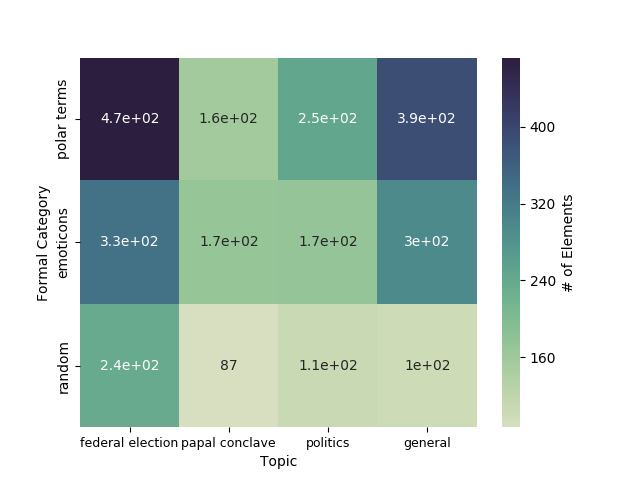
\includegraphics[width=\linewidth]{img/sentiment_stat.png}
  \caption{\texttt{Sentiments}}
\end{subfigure}%
\begin{subfigure}{.5\textwidth}
  \centering
  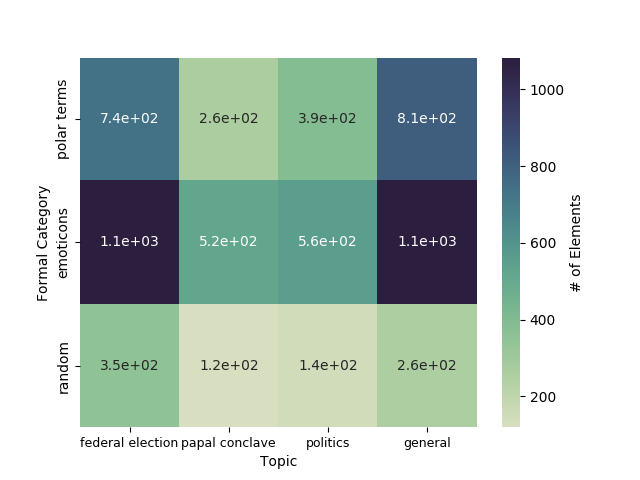
\includegraphics[width=\linewidth]{img/emo-expression_stat.png}
  \caption{\texttt{Emotional expressions}}
\end{subfigure}
}
\caption{Distribution of sentiments and emotional expressions across
  topics and formal categories.}\label{fig:distr}
\end{figure*}

\begin{figure*}[htbp!]
{
\centering
\begin{subfigure}{.5\textwidth}
  \centering
  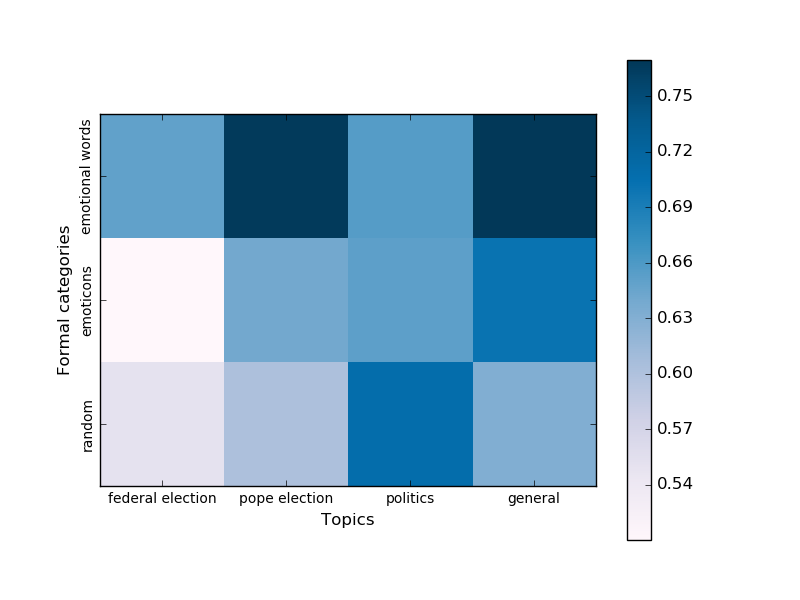
\includegraphics[width=\linewidth]{img/sentiment_agreement.png}
  \caption{\texttt{Sentiments}}
\end{subfigure}%
\begin{subfigure}{.5\textwidth}
  \centering
  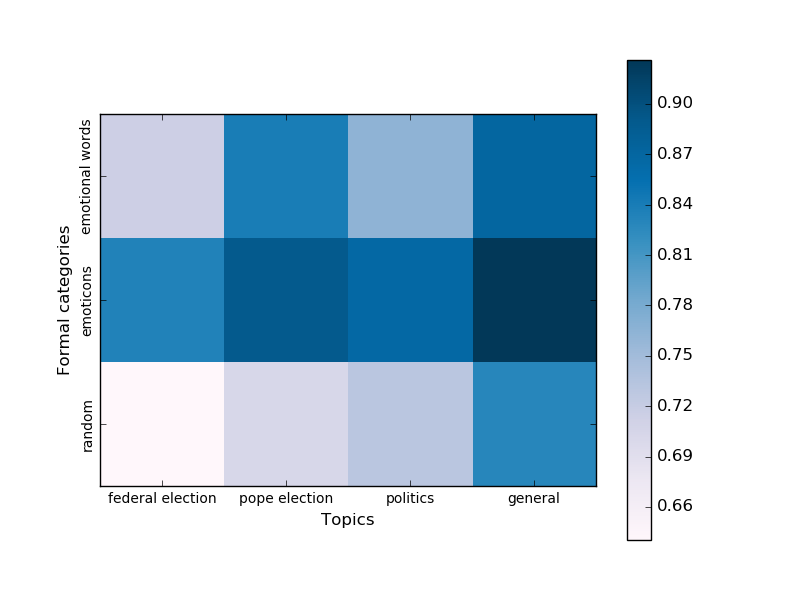
\includegraphics[width=\linewidth]{img/emo-expression_agreement.png}
  \caption{\texttt{Emotional expressions}}
\end{subfigure}
}
\caption{Inter-annotators agreement on sentiments and emotional
  expressions across topics and formal categories.}\label{fig:distr}
\end{figure*}

As can be seen from the scores, reaching a consensus about the
polarities of emotional terms was much easier than agreeing on the
value of this attribute for complete opinions.  Similar to
Example~\ref{example:sent-disagr}, one of the main reasons for these
disagreements were subjective opinions containing smileys, especially
in the cases when the polarity of the emoticon contradicted the
polarity of its preceding sentence, e.g., ``Ich hasse die
Piratenpartei \smiley{}'' (\emph{I hate the Pirate Party {\upshape
    \smiley{}}}).

Finally, to check how the selection criteria that we applied initially
for sampling our corpus affected the final distribution of sentiments
and polar expressions, we generated statistics plots on the
frequencies and agreement level of these elements in the annotated
dataset.  As can be seen from the figures, the stratification
according to topics and formal features has notably influenced both
the number of these elements and the difficulty of their
interpretation.

According to Figure \ref{fig:distr}, federal elections and topically
unfiltered tweets are the ones that contain the major part of the
opinions.  A similar tendency is also observed for emotional
expressions, though, in this case, the formal grouping appears to play
a more important role than topics.  Interestingly enough, the higher
number of polar terms does not necessarily imply a higher number of
targeted sentiments.  We can recognize that from the fact that, even
though most of the polar terms show up in the second row of the plot
(i.e., in microblogs with smileys), the biggest number of opinions
appear in row one (i.e., in tweets containing terms from the SentiWS
lexicon).

Regarding the inter-annotator agreement, we can see that the highest
reliability of annotated opinions is achieved on general tweets taken
from casual everyday conversations.  This group is also the one with
the highest IAA scores for emotional expressions.  A different
situation, however, is observed for these two element types as to the
formal groups of the tweets.  In this case, the first formal category
(i.e., tweets with lexicon terms) appears to comprise messages with
the most reliably annotated sentiments.  For emotional expressions,
however, the emoticons category, again, is the one with the highest
achieved result, whereas, for opinions, the agreement scores in this
row are among the lowest.  This finding suggests that, even though,
smileys are typically recognized as polar entities, the question
whether they relate to something particular in the tweet or rather
express the general mood of the author might often be difficult to
answer.

%% \subsection{Corpus Statistics}\label{subsec:snt:stat}

%% \begin{table}[h]
%%   \centering\small
%%   \caption[Sentiment corpus statistics]{Statistics on the annotated
%%     sentiment corpus.\\ POL = corpus part with discussions about
%%     general politic topics; FE = corpus part describing the federal
%%     election 2013; PE = corpus part with discussions about the Pope
%%     election 2013; GEN = part of the corpus containing tweets with no
%%     particular topic}
%%   \begin{tabular}{|>{\centering}p{0.15\textwidth}|*{4}{>{\centering}p{\oosixthClmnWidth}|}
%%       >{\centering\bfseries}p{\oosixthClmnWidth}|*{4}{>{\centering}p{\oosixthClmnWidth}|}
%%       >{\centering\bfseries}p{\oosixthClmnWidth}|}
%%     \hline

%%     \multirow{2}{*}{\parbox{0.13\textwidth}{\centering Markable Type}}
%%     & \multicolumn{5}{>{\centering}p{7\oosixthClmnWidth}|}{Annotator
%%       1} &
%%     \multicolumn{5}{>{\centering}p{7\oosixthClmnWidth}|}{Annotator
%%       2}\tabularnewline\cline{2-11}

%%     & POL & FE & PE & GEN & Total & POL & FE & PE & GEN &
%%     Total\tabularnewline\hline

%%     Sentiment & 212 & 222 & 163 & 131 & 728 & 317 & 335 & 314 & 305 & 1271
%%     \tabularnewline\hline

%%     Source & 101 & 119 & 68 & 73 & 361 & 114 & 109 & 94 & 85 & 402
%%     \tabularnewline\hline

%%     Target & 229 & 279 & 184 & 151 & 843 & 342 & 369 & 328 & 324 & 1363
%%     \tabularnewline\hline

%%     Emotional Expression & 727 & 689 & 581 & 811 & 2808 & 662 & 669 & 671 & 768 & 2770
%%     \tabularnewline\hline

%%     Intensifier & 16 & 32 & 14 & 44 & 106 & 31 & 35 & 31 & 58 & 155
%%     \tabularnewline\hline

%%     Diminisher & 2 & 4 & 3 & 2 & 11 & 2 & 9 & 4 & 2 & 17
%%     \tabularnewline\hline

%%     Negation & 18 & 15 & 23 & 14 & 70 & 33 & 33 & 31 & 23 & 120
%%     \tabularnewline\hline
%%   \end{tabular}
%%   \label{table:sentiment-agreement-topics}
%% \end{table}


\subsection{Related Work}
\newpage
